\chapter{Introduction}\label{cha:intro}

The goal of this report is to describe the process of design and implementation of the Final Undergraduate Project \textit{"SORELCOM: Design and Development of a semantic geospatial web and mobile application"}.

This project has been carried by Aimar Rodr\'iguez Soto, 4th year student of an undergraduate degree in computer science engineering.

The different chapters that form this document are the following:

TODO

\section{Semantic Web}

\subsection{What is it?}

The semantic web is a extension of the current web in which information is given well-defined meaning, better enabling computers and people to work in cooperation. \cite{berners2001semantic}

The idea behind the semantic web is to bring meaning and structure to the contents of web pages, creating an environment where software agents can roam the web carrying out sophisticated tasks for end users. Thanks to the semantic web, this agents will be able to understand the relationships among the information on a web page, beyond simply identifying certain keywords. 

This machine-readable web of data is based standard languages which allow a uniform representation of the information throughout the different semantic data sources. Through this common infrastructure it is possible to share and process information in a relatively simple way, enabling better solution to the usual problem of searching through the web of information. In short, the Semantic Web attempts to give meaning and structure to the contents on the web, allowing computers to better understand this information to do more useful work.

\subsection{The fundamentals}

The Semantic Web is based on standard formats used for a universal representation and manipulation of data. This standards are the following:

\begin{description}
	\item[RDF:] The Resource Description Framework (RDF) is a standard language for representing information resources in the World Wide Web. It is particularly intended to represent metadata about web resources, however, it by generalizing it can also be used to represent information about things that can be identified on the web. \cite{w3crdf}
	RDF provides a framework for representing information which can be exchanged between application without it loosing its meaning and it is intended for situation in which this information needs to be processed by machines instead of displayed to humans, thus making it fitting for the goals of The Semantic Web.
	The framework is based on identifying resources by using Uniform Resource Identifiers (URIs), and describing them in terms of properties and property values, which enables to represent statements about resources as a graph of nodes and arcs formed by the resources, their properties and their property values. For example, in figure \ref{fig:rdfexample} we can find a RDF graph representing a person named Eric Miller. Note that the resources itself as well as the properties and property values may be identified by URIs.
	\begin{figure}
	  \centering
	  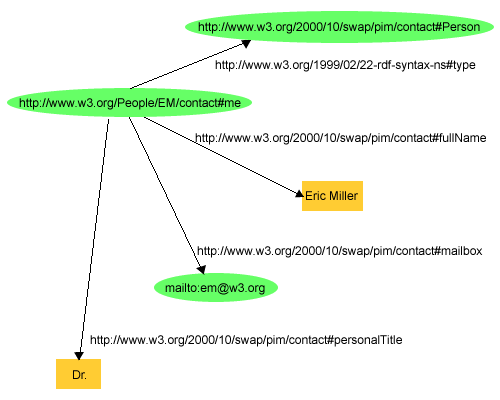
\includegraphics[width=.5\textwidth]{fig/rdfexample}
	  \caption{An RDF graph representing Eric Miller}
	  \captionsetup{font={footnotesize,bf,it}}
	  \caption*{source: \url{http://www.w3.org/TR/2004/REC-rdf-primer-20040210}}
	  \label{fig:rdfexample}
	\end{figure}

\end{description}









